\documentclass[12pt]{article}
\usepackage{fancyhdr}
\usepackage{amsmath, enumitem, tikz, pgf}
\usepackage{amssymb, amsmath, graphicx, amsthm, setspace}
\usetikzlibrary{arrows, automata, positioning}
\usepackage[latin1]{inputenc}
\pagestyle{fancy}

\lhead[lh-even]{\textbf{Michael Vu}}  
\lfoot[lf-even]{} 
\chead[ch-even]{\textbf{CSCI 3500 HW 2}}  
\cfoot[cf-even]{} 
\rhead[rh-even]{February 8, 2018}  
\rfoot[rf-even]{}

\begin{document}

\begin{enumerate}
\item 
	\begin{enumerate}
	\item 
		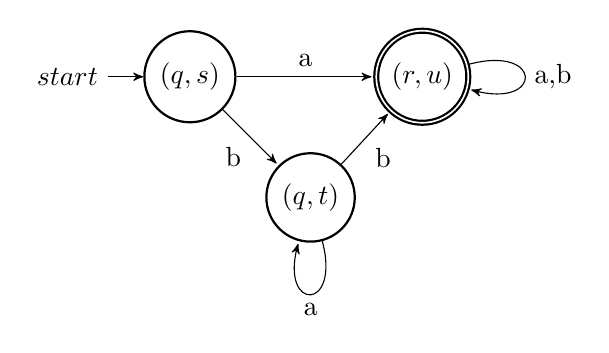
\begin{tikzpicture}
			\tikzset {->, >=stealth', node distance=1.5cm, every state/.style={thick, fill=none}, initial text=$start$ }

			\node[state, initial] 	(A)                  		{$(q,s)$};
			\node[state, accepting]	(B) [right=1.75cm of A]		{$(r,u)$};
			\node[state]			(C) [below right=1cm of A] 	{$(q,t)$};
  
			\draw[every loop]
    		    (A) edge[auto=left] node {a} (B)
				(A) edge[auto=right] node {b} (C)
				(B) edge[loop right] node {a,b} (B)
				(C) edge[loop below] node {a} (C)
				(C) edge[auto=right] node {b} (B);
 
		\end{tikzpicture}
	
	\item
		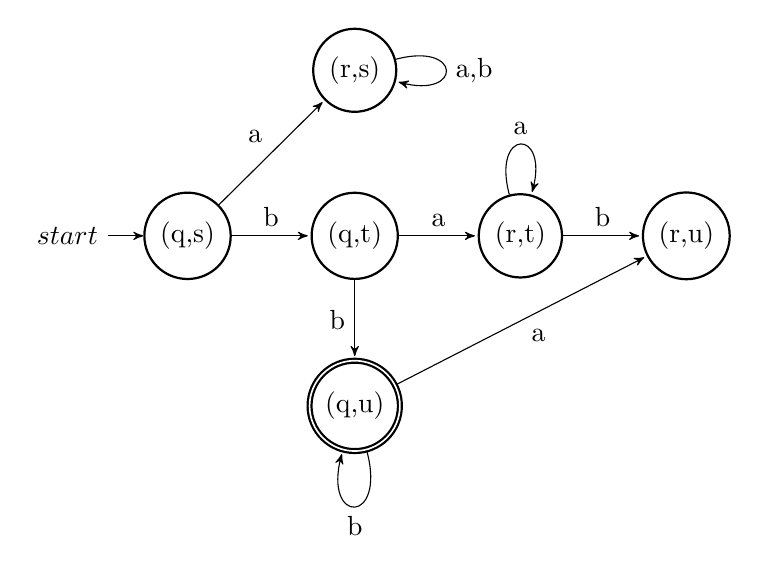
\begin{tikzpicture}
			\tikzset {->, >=stealth', node distance=1cm, every state/.style={thick, fill=none}, initial text=$start$ }
			
			\node[state, initial] (qs) {(q,s)};
			\node[state, right=of qs] (qt) {(q,t)};
			\node[state, above=of qt] (rs) {(r,s)};			
			\node[state, right=of qt] (rt) {(r,t)};
			\node[state, right=of rt] (ru) {(r,u)};
			\node[state, accepting, below= of qt] (qu) {(q,u)};
			
			\draw[every loop]
				(qs) edge[auto=left] node {a} (rs)
				(rs) edge[loop right] node {a,b} (rs)
				(qs) edge[auto=left] node {b} (qt)
				(qt) edge[auto=left] node {a} (rt)
				(rt) edge[loop above] node {a} (rt)
				(rt) edge[auto=left] node {b} (ru)
				(qt) edge[auto=right] node {b} (qu)
				(qu) edge[loop below] node {b} (qu)
				(qu) edge[auto=right] node {a} (ru);
		\end{tikzpicture}
		
	\item
		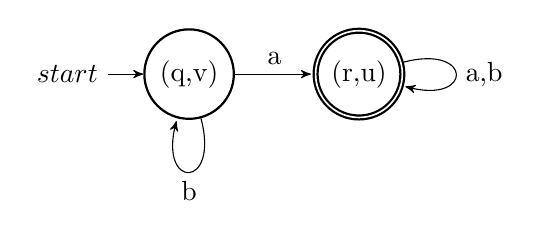
\begin{tikzpicture}
			\tikzset {->, >=stealth', node distance=1cm, every state/.style={thick, fill=none}, initial text=$start$ }
			
			\node[state, initial] (qv) {(q,v)};
			\node[state, accepting, right=of qv] (ru) {(r,u)};
			
			\draw[every loop]
				(qv) edge[auto=left] node {a} (ru)
				(ru) edge[loop right] node {a,b} (ru)
				(qv) edge[loop below] node {b} (qv);
		\end{tikzpicture}
		
	\item 
		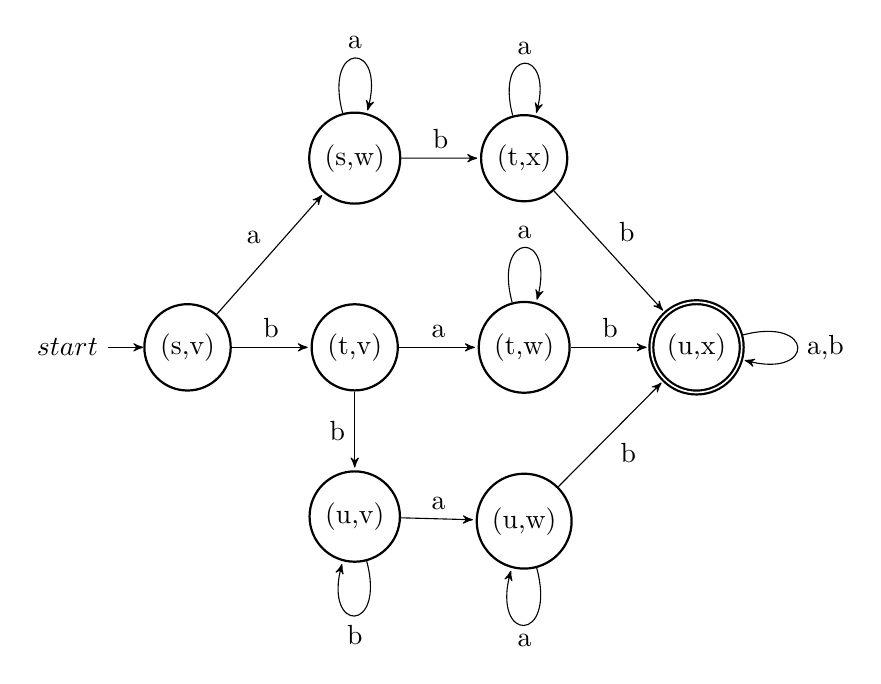
\begin{tikzpicture}
			\tikzset {->, >=stealth', node distance=1cm, every state/.style={thick, fill=none}, initial text=$start$ }
			
			\node[state, initial] (sv) {(s,v)};
			\node[state, right=of sv] (tv) {(t,v)};
			\node[state, right=of tv] (tw) {(t,w)};
			\node[state, accepting, right=of tw] (ux) {(u,x)};
			\node[state, above=1.25cm of tv] (sw) {(s,w)};
			\node[state, above=1.25cm of tw] (tx) {(t,x)};
			\node[state, below=of tv] (uv) {(u,v)};
			\node[state, below=of tw] (uw) {(u,w)};
			
			\draw[every loop]
				(sv) edge[auto=left] node {a} (sw)
				(sw) edge[loop above] node {a} (sw)
				(sw) edge[auto=left] node {b} (tx)
				(tx) edge[loop above] node {a} (tx)
				(tx) edge[auto=left] node {b} (ux)
				(ux) edge[loop right] node {a,b} (ux)
				(sv) edge[auto=left] node {b} (tv)
				(tv) edge[auto=left] node {a} (tw)
				(tw) edge[loop above] node {a} (tw)
				(tw) edge[auto=left] node {b} (ux)
				(tv) edge[auto=right] node {b} (uv)
				(uv) edge[loop below] node {b} (uv)
				(uv) edge[auto=left] node {a} (uw)
				(uw) edge[loop below] node {a} (uw)
				(uw) edge[auto=right] node {b} (ux);
		\end{tikzpicture}
	\end{enumerate}
	
\item See attached C++ file.

\item
	\begin{enumerate}
	\item yes
	\item yes
	\item yes
	\item no
	\item yes
	\end{enumerate}
	
\item
	\begin{enumerate}
	\item
		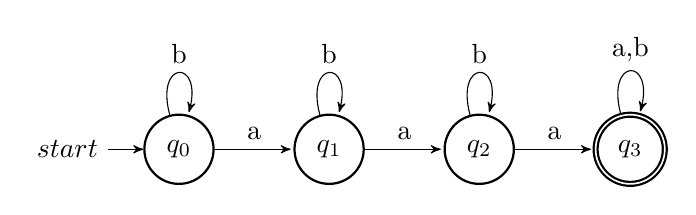
\begin{tikzpicture}
			\tikzset {->, >=stealth', node distance=1cm, every state/.style={thick, fill=none}, initial text=$start$ }
			
			\node[state, initial] (0) {$q_0$};
			\node[state, right=of 0] (1) {$q_1$};
			\node[state, right=of 1] (2) {$q_2$};
			\node[state, accepting, right=of 2] (3) {$q_3$};
			
			\draw[every loop]
				(0) edge[loop above] node {b} (0)
				(0) edge[auto=left] node {a} (1)
				(1) edge[loop above] node {b} (1)
				(1) edge[auto=left] node {a} (2)
				(2) edge[loop above] node {b} (2)
				(2) edge[auto=left] node {a} (3)
				(3) edge[loop above] node {a,b} (3);
		\end{tikzpicture}
		
	\item
		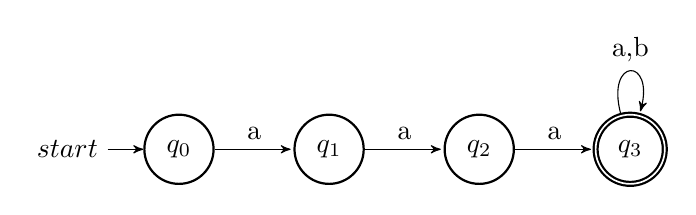
\begin{tikzpicture}
			\tikzset {->, >=stealth', node distance=1cm, every state/.style={thick, fill=none}, initial text=$start$ }
			
			\node[state, initial] (0) {$q_0$};
			\node[state, right=of 0] (1) {$q_1$};
			\node[state, right=of 1] (2) {$q_2$};
			\node[state, accepting, right=of 2] (3) {$q_3$};
			
			\draw[every loop]
				(0) edge[auto=left] node {a} (1)
				(1) edge[auto=left] node {a} (2)
				(2) edge[auto=left] node {a} (3)
				(3) edge[loop above] node {a,b} (3);
		\end{tikzpicture}
		
		
		
	\item
		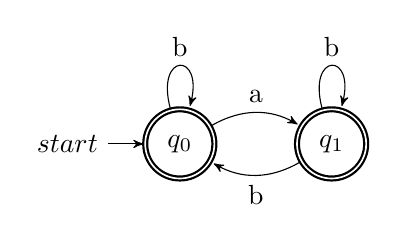
\begin{tikzpicture}
			\tikzset {->, >=stealth', node distance=1cm, every state/.style={thick, fill=none}, initial text=$start$ }
			
			\node[state, initial, accepting] (0) {$q_0$};
			\node[state, accepting, right=of 0] (1) {$q_1$};
			
			\draw[every loop]
				(0) edge[loop above] node {b} (0)
				(0) edge[bend left, auto=left] node {a} (1)
				(1) edge[loop above] node {b} (1)
				(1) edge[bend left, auto=left] node {b} (0);
		\end{tikzpicture}
		
	\item 
		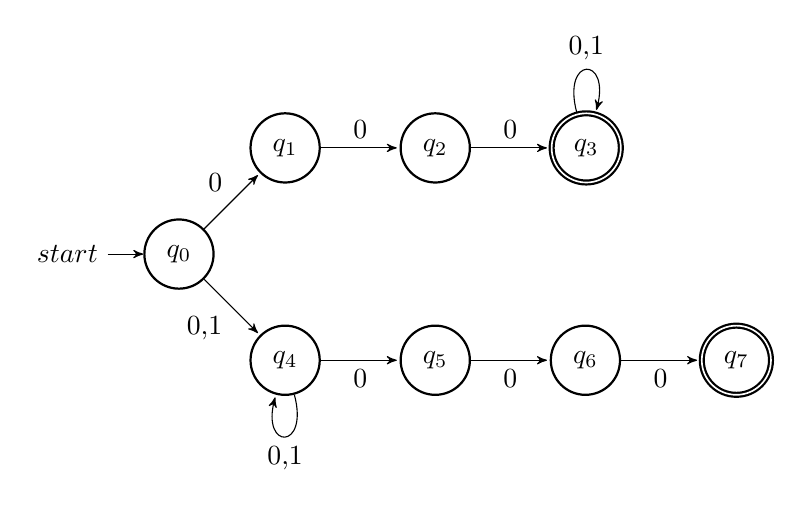
\begin{tikzpicture}
			\tikzset {->, >=stealth', node distance=1cm, every state/.style={thick, fill=none}, initial text=$start$ }
			
			\node[state, initial] (0) {$q_0$};
			\node[state, above right=of 0] (1) {$q_1$};
			\node[state, right=of 1] (2) {$q_2$};
			\node[state, accepting, right=of 2] (3) {$q_3$};
			\node[state, below right=of 0] (4) {$q_4$};
			\node[state, right=of 4] (5) {$q_5$};
			\node[state, right=of 5] (6) {$q_6$};
			\node[state, accepting, right=of 6] (7) {$q_7$};
			
			\draw[every loop]
				(0) edge[auto=left] node {0} (1)
				(1) edge[auto=left] node {0} (2)
				(2) edge[auto=left] node {0} (3)
				(3) edge[loop above] node {0,1} (3)
				(0) edge[auto=right] node {0,1} (4)
				(4) edge[loop below] node {0,1} (4)
				(4) edge[auto=right] node {0} (5)
				(5) edge[auto=right] node {0} (6)
				(6) edge[auto=right] node {0} (7);
		\end{tikzpicture}
	\end{enumerate}
	
	\begin{enumerate}
	\item \{$q_0,q_2$\}
	\item \{$\epsilon$\}
	\item \{$\epsilon$\}
	\item \{$q_0,q_1$\}
	\item \{$q_0,q_1,q_2$\}
	\end{enumerate}
	

\end{enumerate}

\end{document}